\documentclass [xcolor=svgnames, t] {beamer} 
\usepackage[utf8]{inputenc}
\usepackage{booktabs, comment} 
\usepackage[absolute, overlay]{textpos} 
\usepackage{pgfpages}
\usepackage[font=footnotesize]{caption}
\useoutertheme{infolines} 

\AtBeginSection[]{
  \begin{frame}
  \vfill
  \centering
  \begin{beamercolorbox}[sep=8pt,center,shadow=true,rounded=true]{title}
    \usebeamerfont{title}\insertsectionhead\par%
  \end{beamercolorbox}
  \vfill
  \end{frame}
}


%\definecolor{brownbrown}{RGB}{56, 28, 0}
%\definecolor{brownred}{RGB}{228, 0, 43}

%\setbeamercolor{title in head/foot}{bg=brownred, fg=brownbrown}
%\setbeamercolor{author in head/foot}{bg=myuniversity}
\setbeamertemplate{page number in head/foot}{}
\usepackage{csquotes}


\usepackage{amsmath}
\usepackage[makeroom]{cancel}
\usepackage[absolute,overlay]{textpos}
\usepackage{tcolorbox}

%\usepackage{textpos}

\usepackage{tikz}

\usepackage{media9} 

\usetheme{Madrid}
%\definecolor{myuniversity}{RGB}{56, 28, 0}
%\usecolortheme[named=myuniversity]{structure}



\title[Viscosidad]{Clase No.20: Cinem\'atica de los fluidos}
\subtitle{Propiedades cinem\'aticas de los fluidos}
\institute[]{Departamento de Ingenier\'ia Civil y Agr\'icola\\ Facultad de Ingenier\'ia  \\Universidad Nacional de Colombia - Sede Bogot\'a}
\titlegraphic{
\includegraphics[height=2.0cm]{escudoUnal.png}}
\author[LAM]{Luis Alejandro Morales \\ \href{https://lamhydro.github.io}{https://lamhydro.github.io}}


%\institute[]{Department of Earth, Environmental, and Planetary Sciences  \\Brown University}
\date{\today}


\addtobeamertemplate{navigation symbols}{}{%
    \usebeamerfont{footline}%
    \usebeamercolor[fg]{footline}%
    \hspace{1em}%
    \insertframenumber/\inserttotalframenumber
}

\begin{document}
\begin{frame}
\maketitle
\end{frame}


%%%%%%%%%%%%%%%%%%%%%%%%%%%%
\logo{\vspace{-0.2cm}
\includegraphics[height=0.8cm]{escudoUnal.png}~%
}
%%%%%%%%%%%%%%%%%%%%%%%%%%



\begin{frame}
\frametitle{Table of Contents}
\tableofcontents
\end{frame}

\section{Introducci\'on}
\begin{frame}{Introducci\'on}
\begin{block}{Cinem\'atica de los fluidos}
Estudia el movimiento de las part\'iculas de fluido o del fluido como un continuo sin considerar las fuerzas o los momentos actuantes; caracteriza dicho movimiento en funci\'on del espacio y del tiempo.
\begin{textblock*}{5.5cm}(0.3cm,4.3cm) % {block width} (coords)
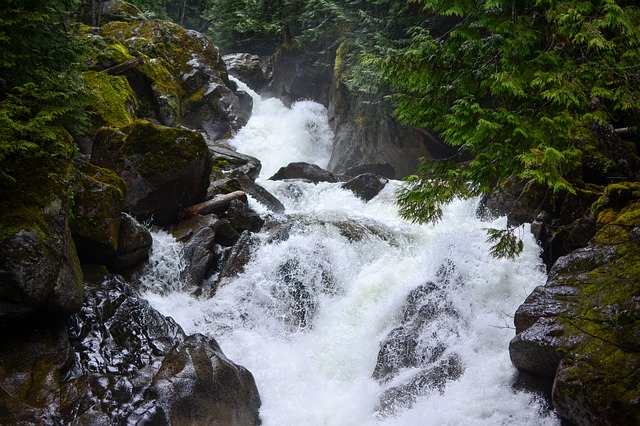
\includegraphics[width=\textwidth]{kine}
\end{textblock*}
\begin{textblock*}{5.5cm}(6.0cm,4.3cm) % {block width} (coords)
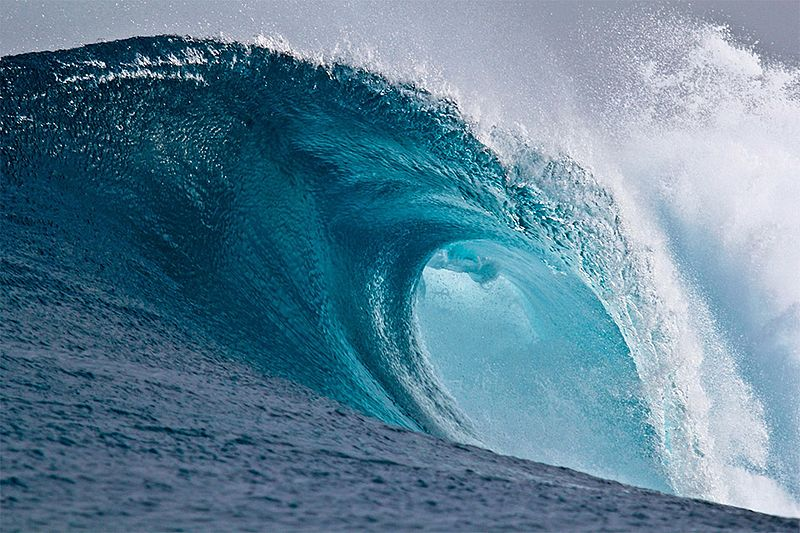
\includegraphics[width=\textwidth]{kine1}
\end{textblock*}
\end{block}
\end{frame} 

\section{Definiciones}
\begin{frame}{Definiciones}
Algunas definiciones importantes del an\'alisis vectorial son:
\begin{block}{Escalar}
Se define por la magnitud que acquiere la cantidad f\'isica. Ejemplos: presi\'on $P$, temperatura $T$, densidad $\rho$
$$
P=f(x,y,z,t) \quad T=f(x,y,z,t) \quad \rho=f(x,y,z,t)
$$
donde $x$, $y$ y $z$ son las coordenadas del espacio 3D y $t$ es el tiempo.
\end{block}
\end{frame}

\begin{frame}{Vector}
\vspace{-0.4cm}
\begin{block}{Vector: Definici\'on}
\begin{columns}
\column{0.4\textwidth}
Es una cantidad que tiene magnitud, direcci\'on y sentido. Ejemplos: velocidad $\vec{U}$ , aceleraci\'on $\vec{a}$, fuerza $\vec{F}$. Un campo de velocidades para un $t=t_1$, puede estar expresado como:
$$
\vec{U}(x,y,z)=u_x \vec{i} + u_y \vec{j} + u_z \vec{k}
$$ 
\column{0.6\textwidth}
\begin{textblock*}{5.5cm}(6.5cm,1.8cm) % {block width} (coords)
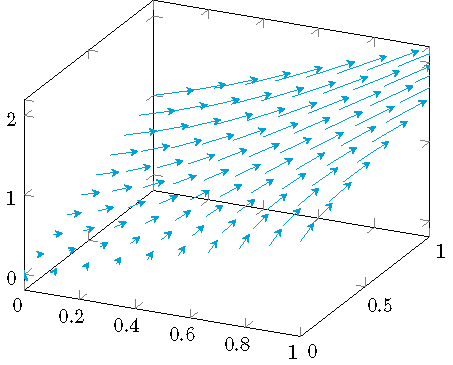
\includegraphics[width=\textwidth]{vecf}
\end{textblock*}
\end{columns}
\vspace{0.5cm}
donde $u_x$, $u_y$ y $u_z$ son las componentes en $x$, $y$ y $z$ del vector $\vec{U}$ respectivamente, en donde cada componente es una $f(x,y,z,t)$. $\vec{i}$, $\vec{j}$ y $\vec{z}$ son los vectores unitarios (de magnitud 1) para $x$, $y$ y $z$, respectivamente. 
\end{block}
\end{frame}

\begin{frame}{Vector}
\vspace{-0.5cm}
\begin{block}{Vector: Operaciones}
Entre dos vectores $\vec{A}$ y $\vec{B}$ es posible efectuar dos tipos de productos:
\begin{enumerate}
\item \emph{Producto escalar o punto}
\vspace{0.3cm}
$$
\vec{A}\cdot \vec{B} = AB \cos \theta
$$
\begin{textblock*}{3cm}(9cm,2.68cm) % {block width} (coords)
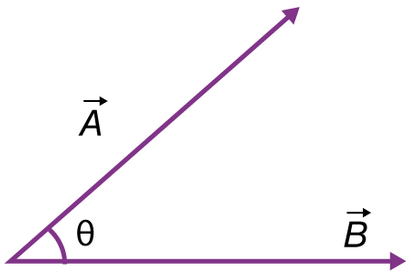
\includegraphics[width=\textwidth]{pes}
\end{textblock*}
donde $\theta$ es el angulo formado por los dos vectores. De acuerdo con esto $\vec{i} \cdot \vec{i} = \vec{j} \cdot \vec{j}= \vec{k} \cdot \vec{k} = 1$, mientras, por ejemplo, $\vec{i} \cdot \vec{j} = \vec{j} \cdot \vec{k} =\vec{i} \cdot \vec{k} = 0$.
\item \emph{Producto vectorial o cruz}
$$
\vec{A} \times \vec{B} = \vec{n}AB \sin \theta
$$
\begin{textblock*}{3cm}(9cm,5.8cm) % {block width} (coords)
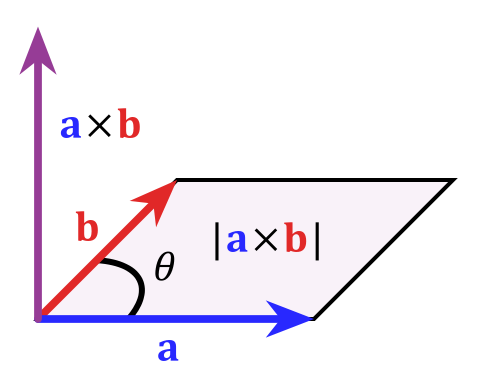
\includegraphics[width=\textwidth]{crop}
\end{textblock*}
donde $\vec{n}$ es el vector unitario perpendicular la plano definido por $\vec{A}$ y $\vec{B}$. De este producto se deriva que $i \times j=k$,$j \times k=i$,$k \times i = j$, $i \times k=-j$ 
\end{enumerate}
\end{block}
\end{frame}


\begin{frame}{Vector: Operadores vectoriales}
\begin{block}{Operador nabla $\nabla$}
Vector simb\'olico que se aplica a cantidades \emph{escalares} y \emph{vectoriales}, se define como:
\begin{equation}
\vec{\nabla} = \frac{\partial }{\partial x}\vec{i} + \frac{\partial }{\partial y}\vec{j} + \frac{\partial }{\partial z}\vec{k}
\label{nb}
\end{equation}
\end{block}
\begin{block}{Gradiente de una funci\'on}
Si el operador $\nabla$ se aplica a una funci\'on escalar $\phi$, se obtiene un vector gradiente definido como:
\begin{equation}
\vec{\nabla} \phi = \frac{\partial \phi}{\partial x}\vec{i} + \frac{\partial \phi}{\partial y}\vec{j} + \frac{\partial \phi}{\partial z}\vec{k}
\label{phi}
\end{equation}
\end{block}
\end{frame}

\begin{frame}{Vector: Operadores vectoriales}
\begin{block}{Divergencia}
Si el operador $\nabla$ aplica a un vector $\vec{U}$ mediante producto punto, se obtiene un escalar conocido como la divergencia de $\vec{U}$, que se expresa como:
\begin{equation}
\vec{\nabla} \cdot \vec{U} = \left[ \frac{\partial }{\partial x}\vec{i} + \frac{\partial }{\partial y}\vec{j} + \frac{\partial }{\partial z}\vec{k} \right] [u\vec{i}+v\vec{j}+w\vec{k}] = \frac{\partial u}{\partial x}+\frac{\partial v}{\partial y}+\frac{\partial w}{\partial z}
\label{di1}
\end{equation}
Note que $\nabla \cdot \vec{U} \ne \vec{U} \cdot \nabla$, entonces:
\begin{equation*}
\vec{U} \cdot \nabla  = [u\vec{i}+v\vec{j}+w\vec{k}] \left[ \frac{\partial }{\partial x}\vec{i} + \frac{\partial }{\partial y}\vec{j} + \frac{\partial }{\partial z}\vec{k} \right]  = u\frac{\partial}{\partial x}+v\frac{\partial}{\partial y}+w\frac{\partial}{\partial z}
\end{equation*}
\end{block}
\end{frame}

\begin{frame}{Vector: Operadores vectoriales}
\vspace{-0.5cm}
\begin{block}{Rotacional}
Es el producto cruz entre el operador $\nabla$ y un vector $\vec{U}$, se obtiene un vector conocido como el rotacional de $\vec{U}$, que se expresa como:
$$
\vec{\nabla} \times \vec{U} = \left[ \frac{\partial }{\partial x}\vec{i} + \frac{\partial }{\partial y}\vec{j} + \frac{\partial }{\partial z}\vec{k} \right] x [u\vec{i}+v\vec{j}+w\vec{k}] = \begin{vmatrix} \vec{i} & \vec{j} & \vec{k} \\ \frac{\partial}{\partial x} & \frac{\partial}{\partial y} & \frac{\partial}{\partial z} \\ u & v & w \end{vmatrix} 
$$
\begin{equation}
\vec{\nabla} \times \vec{U} = \left ( \frac{\partial w}{\partial y}-\frac{\partial v}{\partial z}\right )\vec{i} + \left ( \frac{\partial u}{\partial z}-\frac{\partial w}{\partial x}\right )\vec{j} + \left ( \frac{\partial v}{\partial x}-\frac{\partial u}{\partial y}\right )\vec{k}
\label{rot}
\end{equation}
\begin{textblock*}{3.5cm}(5cm,6.1cm) % {block width} (coords)
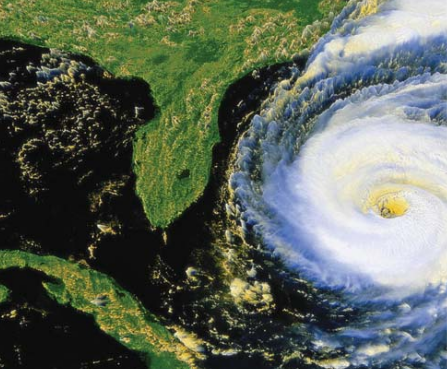
\includegraphics[width=\textwidth]{rota}
\end{textblock*}
\end{block}
\end{frame}

\begin{frame}{Vector: Operadores vectoriales}
\vspace{-0.5cm}
\footnotesize
\begin{block}{Laplaciano}
Se define como:
\begin{equation}
\vec{\nabla} \cdot \vec{\nabla} = \nabla^2 = \left[ \frac{\partial^2 }{\partial x^2} + \frac{\partial^2}{\partial y^2} + \frac{\partial^2}{\partial z^2} \right]
\label{lap}
\end{equation}
Si $\nabla^2$ se aplica sobre una funci\'on escalar $\phi$, se obtiene el escalar:
\begin{equation}
\nabla^2 \phi = \left[ \frac{\partial^2 \phi}{\partial x^2} + \frac{\partial^2 \phi}{\partial y^2} + \frac{\partial^2 \phi}{\partial z^2} \right]
\label{lap2}
\end{equation}
Si $\nabla^2$ se aplica sobre un vector  $\vec{U}$ (e.g. velocidad), se obtiene el vector:
$$
\nabla^2 \vec{U} = \left[ \frac{\partial^2}{\partial x^2} + \frac{\partial^2}{\partial y^2} + \frac{\partial^2}{\partial z^2} \right][u\vec{i}+v\vec{j}+w\vec{k}]
$$
$$
\nabla^2 \vec{U} = \left[ \frac{\partial^2 u}{\partial x^2} + \frac{\partial^2 u}{\partial y^2} + \frac{\partial^2 u}{\partial z^2} \right]\vec{i} + \left[ \frac{\partial^2 v}{\partial x^2} + \frac{\partial^2 v}{\partial y^2} + \frac{\partial^2 v}{\partial z^2} \right]\vec{j} + \left[ \frac{\partial^2 w}{\partial x^2} + \frac{\partial^2 w}{\partial y^2} + \frac{\partial^2 w}{\partial z^2} \right]\vec{k}
$$
\vspace{0.4cm}
\begin{equation}
\nabla^2 \vec{U} =\vec{i} \nabla^2 u + \vec{j} \nabla^2 v + \vec{k} \nabla^2 w
\label{lap3}
\end{equation}
\end{block}
\end{frame}


\begin{frame}{Campo escalar}
\begin{block}{Campo escalar}
Un escalar $\phi$ es funci\'on de las coordenadas espaciales $x$, $y$ y $z$ o del vector de posici\'on $\vec{r}$ del punto $P(x,y,z)$; $\vec{r}$ une al origen del sistema de referencia con  $P$. Es posible entonces escribir:
$$
\phi = \phi(x,y,z) = \phi(P)=\phi(\vec{r})
$$
Por lo tanto un campo escalar queda definido si para cada punto $P$ existe un \'unico valor de $\phi$ exigi\'endose que la funci\'on $\phi(x,y,z)$ sea continua y derivable en el espacio. El espacio geom\'etrico para el cual m\'ultiple puntos $(x,y,z)$ tienen el mismo valor de $\phi$ se denomina \alert{superficie equipotencial}. Si $\phi=f(x,y)$, el lugar geom\'etrico de todos los punto con igual valor $\phi$ es una \alert{linea equipotencial}. La presi\'on en un fluido es un ejemplo de un campo escalar.
\end{block}
\end{frame}

\begin{frame}{Campo vectorial y potencial}
\vspace{-0.5cm}
\begin{block}{Campo vectorial}
Si un vector $\vec{A}$ es funci\'on de su posici\'on $(x,y,z)$ en el espacio, se puede escribir que:
$$
\vec{A} = \vec{A}(x,y,z) = \vec{A}(P) = \vec{A}(\vec{r}) = a(x,y,z)\vec{i} + b(x,y,z)\vec{j} + c(x,y,z)\vec{k}
$$
donde $a$ $b$ y $c$ son las componentes de $\vec{A}$. Por lo tanto un \alert{campo vectorial} esta definido si existe un valor de $\vec{A}$ en capa punto $P(x,y,z)$. La velocidad de un fluido $\vec{U}$ es un ejemplo de un campo vectorial.
\end{block}
\begin{block}{Campo potencial}
Un campo potencial es aquel en el que:
$$
\vec{U} = \vec{\nabla} \phi = \frac{\partial \phi}{\partial x}\vec{i} + \frac{\partial \phi}{\partial y}\vec{j} + \frac{\partial \phi}{\partial z}\vec{k}
$$
en donde $\vec{U}$ es la velocidad y $\phi$ es una funci\'on escalar.
\end{block}
\end{frame}

\begin{frame}{Concepto de flujo de un campo vectorial y de circulaci\'on de un vector}
\vspace{-0.5cm}
\begin{block}{Concepto de flujo de un campo vectorial}
Sup\'ongase que existe un campo vectorial $\vec{A}=\vec{A}(\vec{r})$ y una superficie $S$ delimitada por una linea $L$. Un diferencial $dS$  esta definido por el vector unitario $\vec{n}$ perpendicular a $dS$. Asi el flujo del vector $A$ a trav\'es de la superficie $S$ es:
$$
\psi = \int_S \vec{A} \cdot \vec{n}dS = \int_S \vec{A} \cdot dS 
$$
\end{block}
\vspace{-0.23cm}
\begin{block}{Concepto de circulaci\'on de un vector}
La circulaci\'on de un vector $\vec{A}$ a lo largo de la linea $L$ est\'a definida como:
$$
\Gamma = \int_L \vec{A} \cdot d\vec{L}
$$
Si $\vec{A}$ representa un campo de fuerza $\vec{F}$, $\Gamma$ representa el trabajo mec\'anico realizado por $\vec{F}$.
\end{block}
\end{frame}

\section{Teorema de Gauss de la divergencia}
\begin{frame}{Teorema de Gauss de la divergencia}
\vspace{-0.5cm}
\begin{block}{Teorema de Gauss de la divergencia}
La integral de la divergencia de un campo escalar o vectorial $A$ tomada sobre un volumen $V$ es igual a la integral de la componente normal de este campo tomada sobre la superficie $S$ que encierra el volumen $V$. Esto se expresa como:
\begin{equation}
\int_V \vec{\nabla} \cdot A dV = \int_S \vec{A} \vec{n}  dS 
\label{tga}
\end{equation}
El teorema permite transforma integrales de volumen en integrales de superficie o viceversa. Su importancia f\'isica radica en que sirve para calcular el flujo neto a trav\'es de una superficie cerrada de una cantidad escalar o vectorial.
\end{block}
\begin{textblock*}{4cm}(5cm,6.4cm) % {block width} (coords)
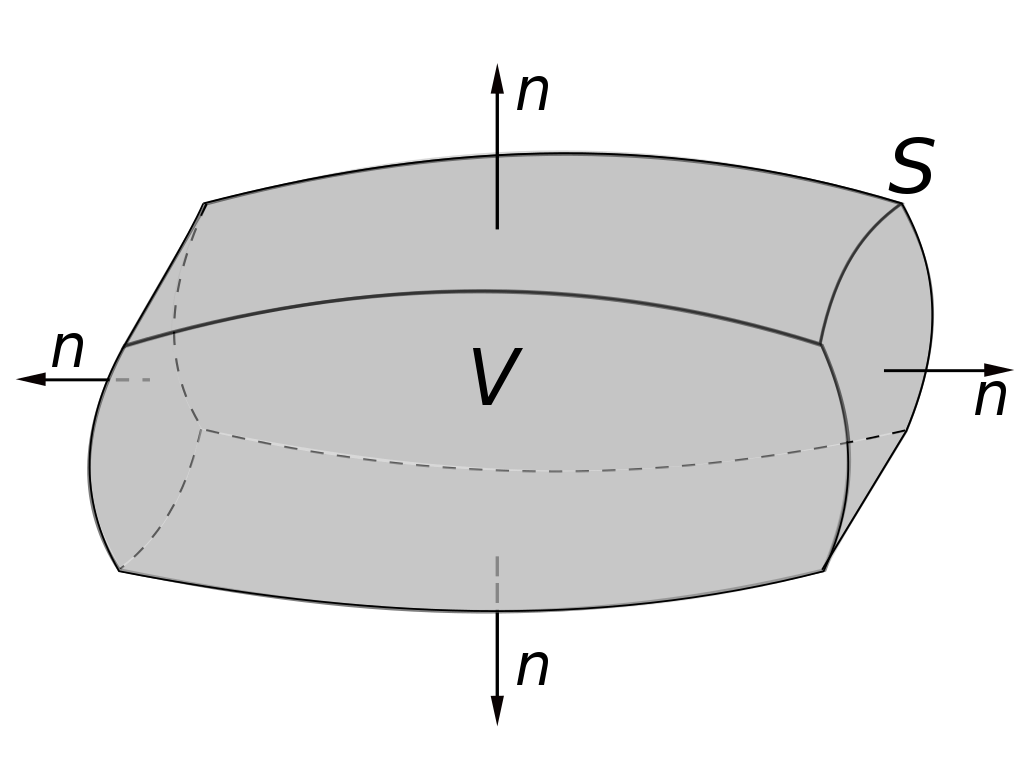
\includegraphics[width=\textwidth]{gau}
\end{textblock*}
\end{frame}

\section{Teorema de Stokes}
\begin{frame}{Teorema de Stokes}
\begin{block}{Teorema de Stokes}
La integral de linea de la componente tangencial de un vector $A$ a lo largo de una curva cerrada $C$ es igual a la integral de superficie de la componente normal del rotacional de $A$ extendida a una superficie cualquiera que tenga por contorno la curva $C$. Esto se expresa como:
\begin{equation}
\int_C A \cdot dl = \int_S \vec{n}(\nabla \times A)dS
\label{tst}
\end{equation}
donde $dl$ es un pequeno desplazamiento a lo largo de la curva $C$ y $dS$ es es un pequeno vector de area.
\end{block}
\begin{textblock*}{5cm}(4cm,6.8cm) % {block width} (coords)
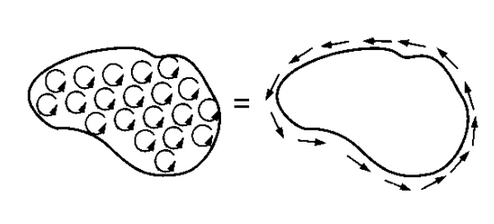
\includegraphics[width=\textwidth]{sto}
\end{textblock*}
\end{frame}


\end{document}

